\documentclass{report}
\usepackage{graphicx} % Required for inserting images
\usepackage{float}
\usepackage{hyperref}

\usepackage[italian]{babel}
\usepackage[italian]{cleveref}

\setcounter{tocdepth}{3}
\setcounter{secnumdepth}{3}

\title{
\normalsize{Corso di Sistemi Embedded e Internet of Things}\\
\Huge{Smart Temperature Monitoring System}\\
\vspace{0.75em}
\large{Progettazione e costruzione di un \textit{sistema di controllo di temperatura} ed implementazione di una Macchina a Stati Finiti}
}
\author{Luca Ponseggi \and Jacopo Turchi \and Luca Venturini \and Federico Bagattoni}
\date{\today}

\begin{document}

\maketitle

\tableofcontents
\newpage
\section*{Introduzione}
\par{
L'obbiettivo del progetto finale del corso è costruire ed implementare un sistema di monitoraggio della temperatura che cambia in autonomia l'apertura di una finestra controllata da servo motore. Il sistema consente all'utente di aprire manualmente la finestra e fornisce un interfacia web per la visualizzazione dei dati.
}
\par{
Per lo sviluppo verrà utilizzata la piattaforma \textbf{Arduno Uno} e \textbf{ESP-32} con sensore di temperatura. Per quanto riguarda il backend viene utilizzato il framework \href{https://vertx.io/}{Vertx.io} consigliato a lezione.
}

\chapter{Unità di controllo}
\par {
Il sistema di controllo, codificato in Java, è totalmente basato sul framework Vertx.io che consente la creazione di più unità di elaborazione dette \textit{verticles} (\textit{vertici}) che vengono eseguite ciascuna in un thread separato. \\
Per far comunicare ciascun vertice il framework fornisce l'\textit{Event Bus}, un sistema di messaggistica che permette di scambiare messaggi tra vertici in diverse maniere (request-reply, publish-subscribe...). L'Event Bus viene usato per la trasmissione dei dati all'interno del modello. 
}
\par {
Il vantaggio dei vertici è quello di permettere comunicazione asincrona tra il backend e le varie componenti, delegando al framework ed alla JVM lo scheduling, la concorrenza e la gestione delle comunicazioni. \\
Infatti ogni vertice rappresenta una task o un componente del modello.
}
\par {
Il modello conserva i dati in apposite classi ed un vertice implementato come una macchina a stati finiti e prende decisioni riguardo al comportamento del sistema. Altri vertici servono solo per scambiare comunicazioni tra le altre unità del sistema ed il backend.
}

\section{Task del sistema}

\par{
L'architettura prevede x tasks: 
}
\begin{itemize}
    \item {
    \textbf{Backend verticle}: questo vertice è l'automa principale dell'unità di controllo. Esso prende decisioni e cambia il suo stato in base alla temperatura rilevata e modifica conseguentemente anche l'apertura della finestra. E' implementato come una macchina a stati finiti di cui si può vedere il comportamento dettagliato nell'immagine.
    \begin{figure}[H]
        \centering
        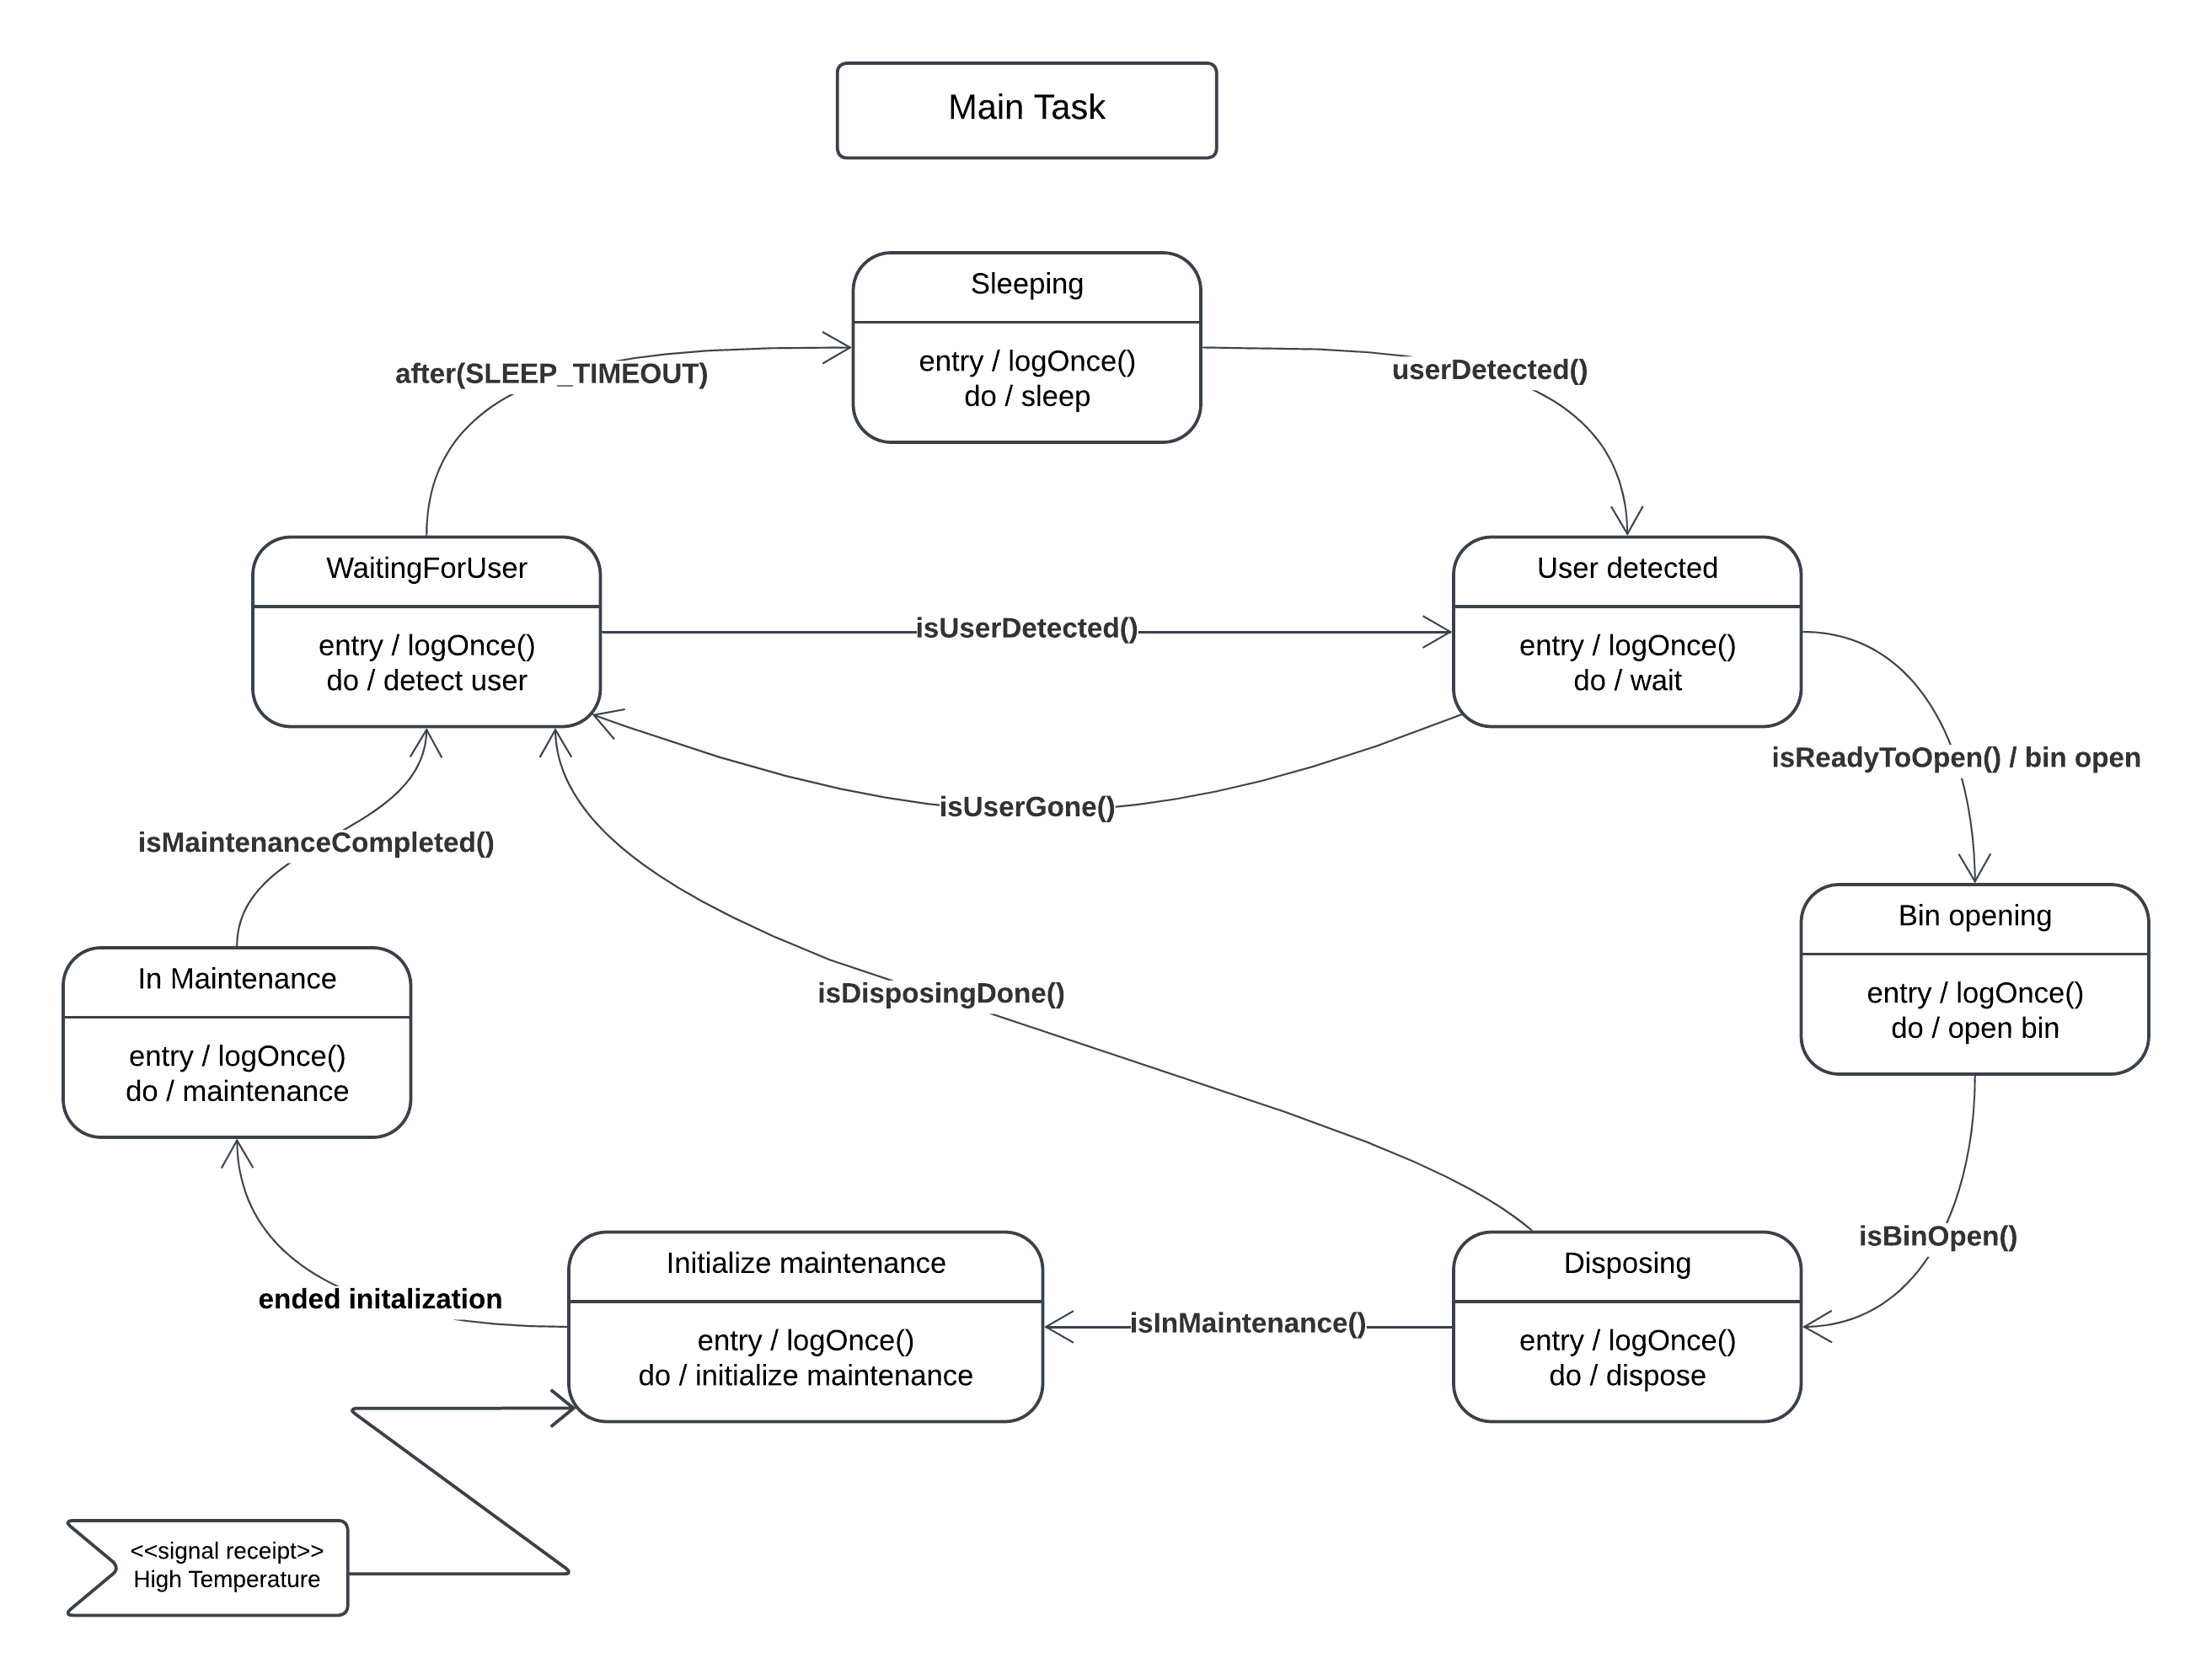
\includegraphics[width=\linewidth]{assignment-03/img/Diagrammi per IOT - MainTask.png}
        \caption{diagramma degli stati di \textit{Main task}}
        \label{fig:main-task}
    \end{figure}
    }
    \item {
    \textbf{Smart Thermometer Verticle}: contenuto in BackendVerticle esso funge da endpoint per i valori di temperatura che arrivano, attraverso l'Event Bus, dal componente deputato alla comunicazione MQTT. Questa classe è l'astrazione locale del sistema di misurazione di temperatura ESP-32.
    \begin{figure}[H]
        \centering
        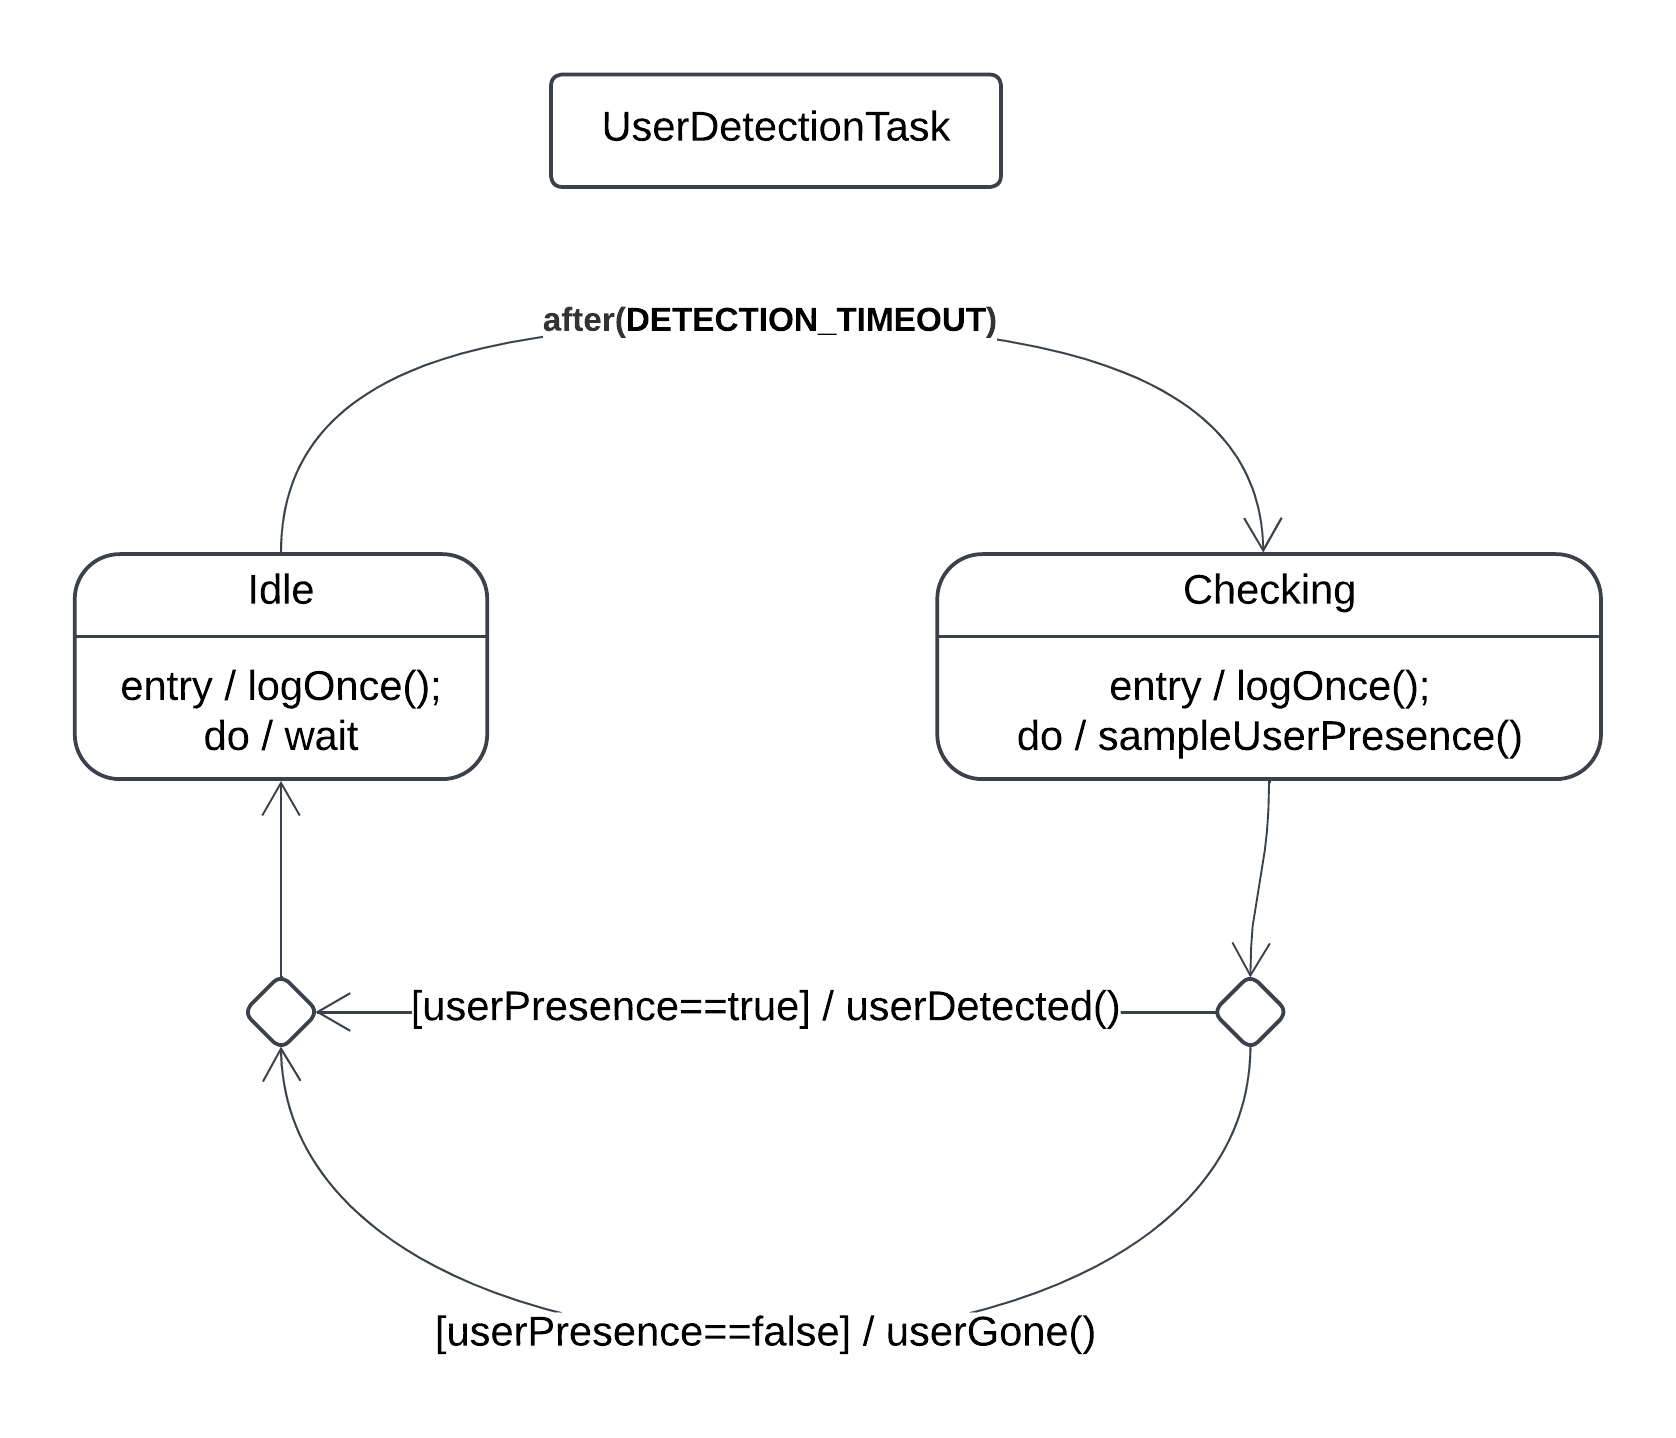
\includegraphics[width=0.7\linewidth]{assignment-02/img/Diagrammi per IOT - User DetectionTask.png}
        \caption{diagramma degli stati di \textit{User detection task}}
        \label{fig:detection-task}
    \end{figure}
    }
    \item {
    \textbf{Smart Window Verticle}: questa classe è l'astrazione del sistema di controllo della finestra Arduino. Conserva ampiezza della finestra ed invia il nuovo parametro quando viene modificato. Questo vertice fa anch'esso parte di BackendVerticle.
    \begin{figure}[H]
        \centering
        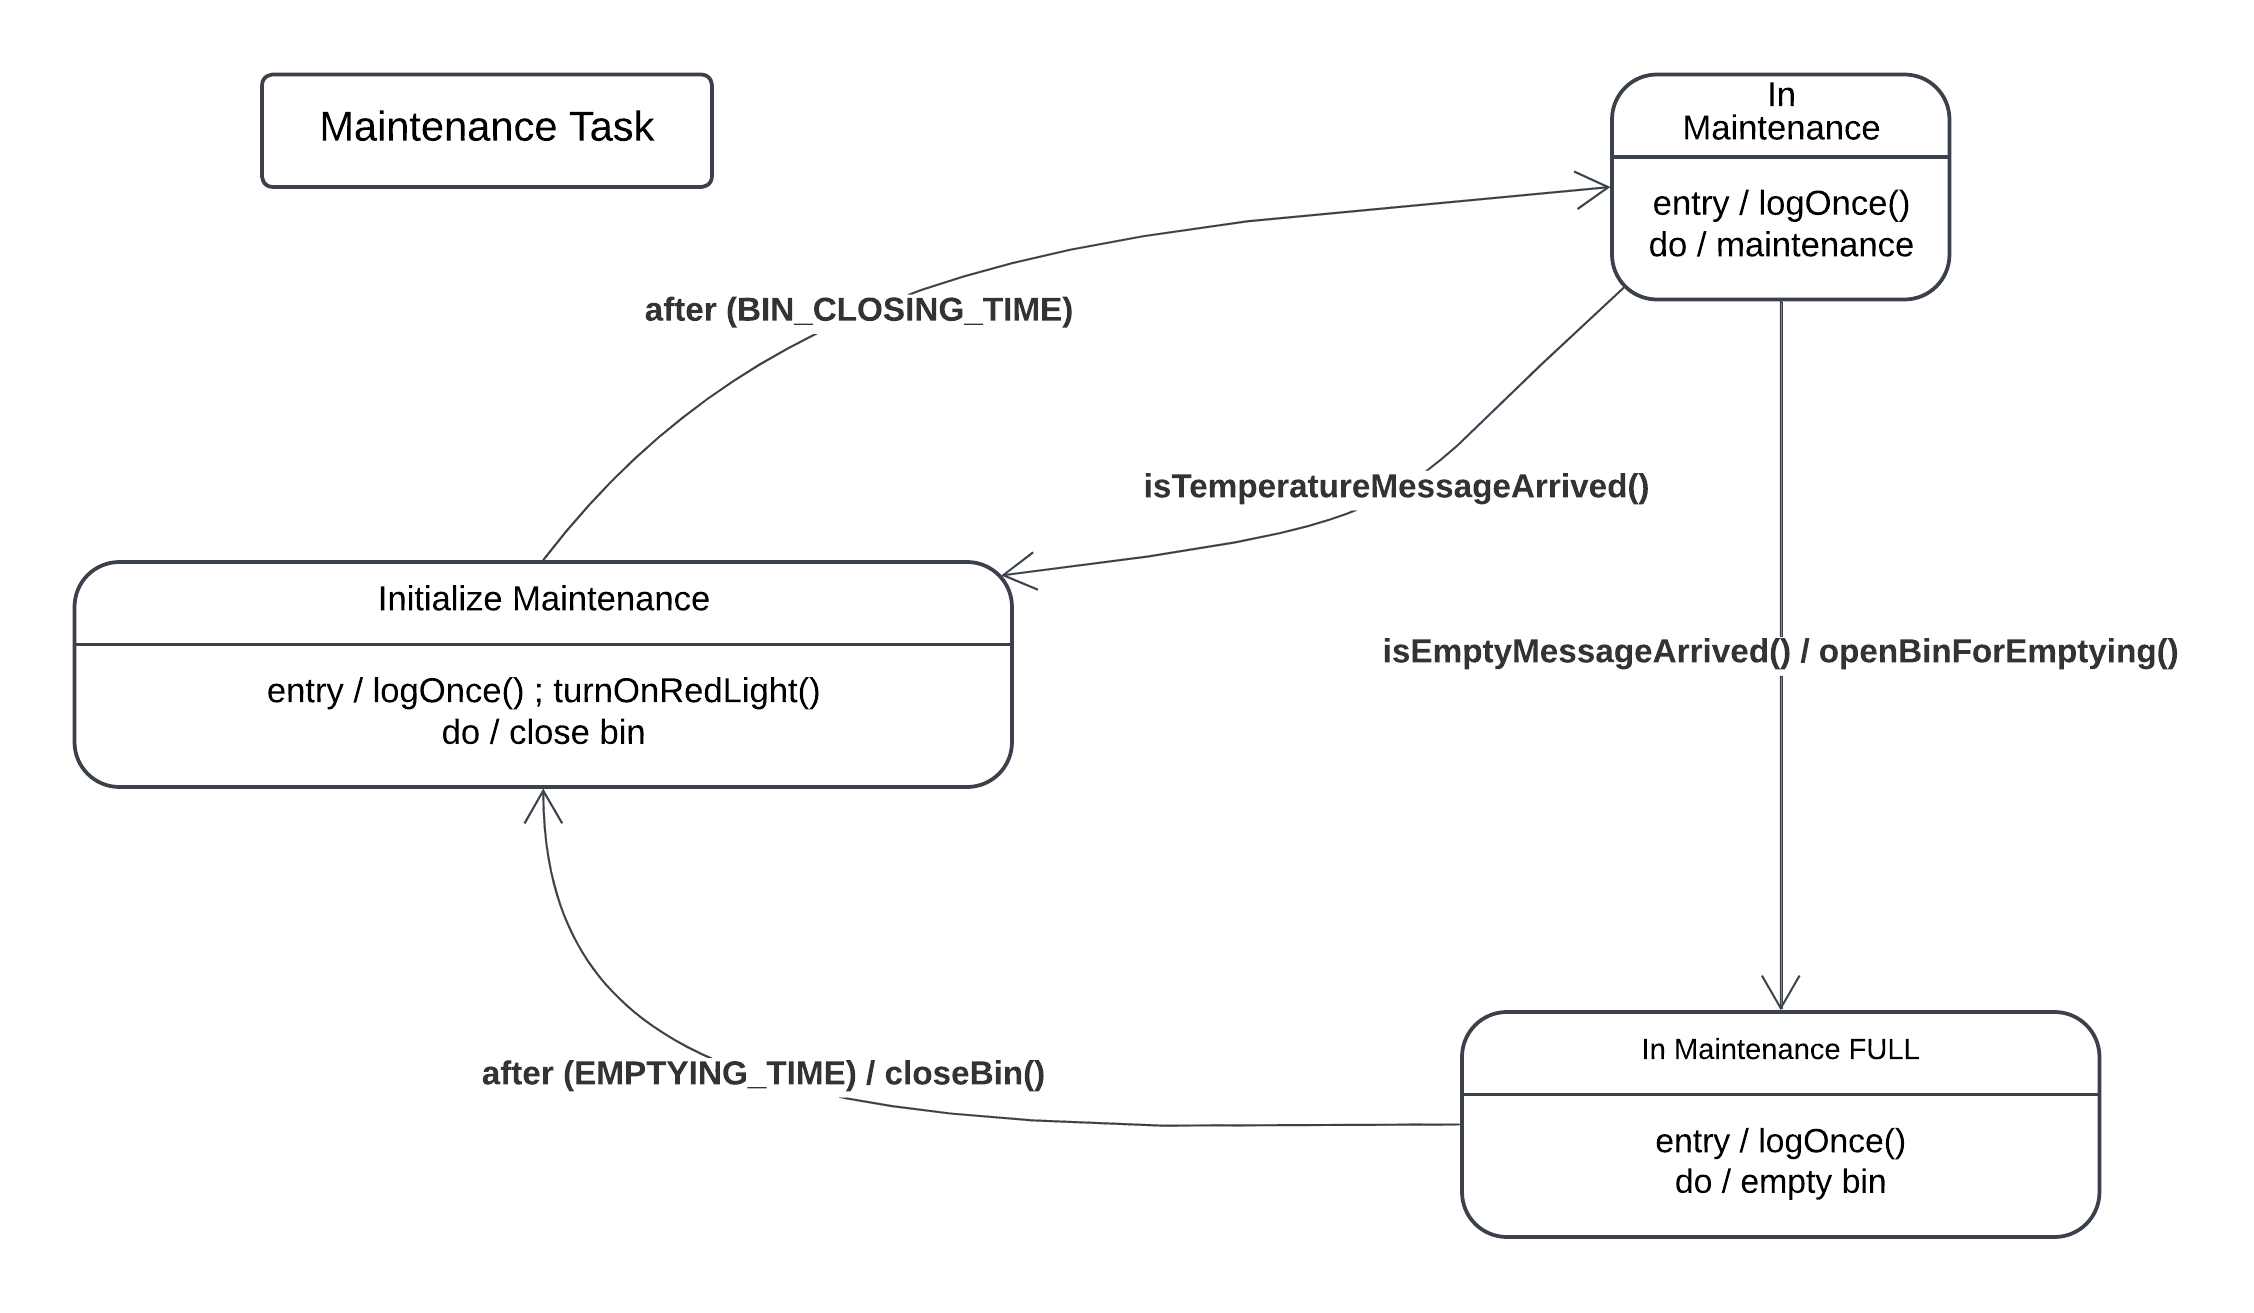
\includegraphics[width=\linewidth]{assignment-02/img/Diagrammi per IOT - MaintenanceTask.png}
        \caption{diagramma degli stati di \textit{Maintenance task}}
        \label{fig:maintenance-task}
    \end{figure}
    }
    \item {
    \textbf{Smart Dashboard Verticle}: rappresenta la dashboard web in cui vengono visualizzati i dati. Questa non è particolarmente complicata perché i dati vengono richiesti e forniti tramite l'utilizzo di funzionalità del framework quindi non vi è nessuna particolare astrazione. 
    }
\end{itemize}

\section{La Macchina a Stati Finiti}
Come indicato nel capitolo precedente la \hyperref[fig:main-task]{Main task} gestisce il funzionamento dell'intero sistema. Questa è una macchina a stati finiti che reagisce alla variazione dei parametri del sistema e cambia il suo stato di conseguenza. 

\section{Funzionamento specifico}
\par {
La MSF ha 6 stati. All'avvio è posizionata nello stato \textbf{IDLE}, questo stato è usato come passaggio sia all'inizializzazione sia quando si passa da manuale ad automatico. Infatti questo stato permette di decidere in che stato posizionarsi.
}
\subsection{La modalità automatica}

\par{
Gli stati corrispondenti alla modalità automatica sono \textbf{NORMAL}, \textbf{HOT}, \textbf{TOO HOT}, \textbf{ALARM}. La macchina salta da uno stato all'altro in base alle soglie di temperatura in cui è configurata. \\
Nello stato \textbf{HOT} modifica l'apertura della finestra in base alla temperatura. \\
Rimane indefinitvamente nello stato \textbf{ALARM} di finché il sistema non viene ripristinato.
}
\subsection{La modalità manuale}
La modalità manuale consiste di due stati in quanto \textit{una discrepanza con la descrizione delle specifiche creava un conflitto di interessi tra i componenti del sistema}. 
Gli stati sono \textbf{MANUAL ARDUINO} e \textbf{MANUAL DASHBOARD} che rappresentano la modalità manuale per ciascun componente che può abilitarla. Questo facilita la sincronizzazione ed evita che i sistemi, entrambi in manuale, abbiamo comportamenti non indicati nelle specifiche. \\
\begin{itemize}
    \item Quando il sistema è in \textbf{MANUAL ARDUINO} il sotto sistema Arduino è in controllo dell'apertura della finestra e la dashboard web si comporterà come fosse in modalità automatica (esattamente come prima  che Arduino entrasse in modalità manuale)
    \item Quando il sistema è in \textbf{MANUAL DASHBOARD} il sotto sistema della dashboard web è in controllo dell'apertura della finestra. Analogamente al punto precedente il sistema Arduino è ignaro della situazione e si comporta come se fosse in modalità automatica. 
\end{itemize}
L'implementazione che abbiamo fornito è la nostra interpretazione delle specifiche permettendo la massima fedeltà per i due sottisistemi Web e Arduino aggiungendo un solo stato al sistema senza violare nessuna altra regola. 

\section{Schema dell'unità di controllo}
Di seguito viene fornito lo schema dell'unità di controllo.
%
%
\chapter{Dashboard}
Nel seguente capitolo viene mostrata la dashboard realizzata in Java visualizzata al computer. L'interfaccia mostra tre informazioni principali:
\begin{itemize}
    \item \textbf{Status}: indica lo stato corrente del sistema (ad esempio, \textit{Waiting}, ossia in attesa di nuovi rifiuti).
    \item \textbf{Temperature}: visualizza la temperatura interna del contenitore per verificare che sia entro i limiti di sicurezza.
    \item \textbf{Fill level}: mostra il livello di riempimento del contenitore, utile per sapere quando è necessario svuotarlo.
\end{itemize}
La dashboard presenta anche due pulsanti funzionali:
\begin{itemize}
    \item \textbf{Empty}: utilizzato per svuotare il contenitore una volta che è pieno.
    \item \textbf{Restore}: serve a ripristinare il sistema dopo che è stato rilevato un problema, come una temperatura elevata.
\end{itemize}
Questa GUI comunica con il sistema Arduino tramite una connessione seriale per gestire in tempo reale le operazioni di controllo e monitoraggio del sistema.
\begin{figure}[H]
    \centering
    \includegraphics[width=\linewidth]{assignment-03/img/javaGui.png}
    \caption{Interfaccia utente}
    \label{fig:GUI}
\end{figure}


\chapter{Circuito}
Di seguito viene riportato lo schema del circuito utilizzato. Si rammenta che potrebbero esserci delle discrepanze tra il circuito realmente realizzato e quello rappresentato in immagine a causa di differenze funzionali nel software di disegno.
\begin{figure}[H]
    \centering
    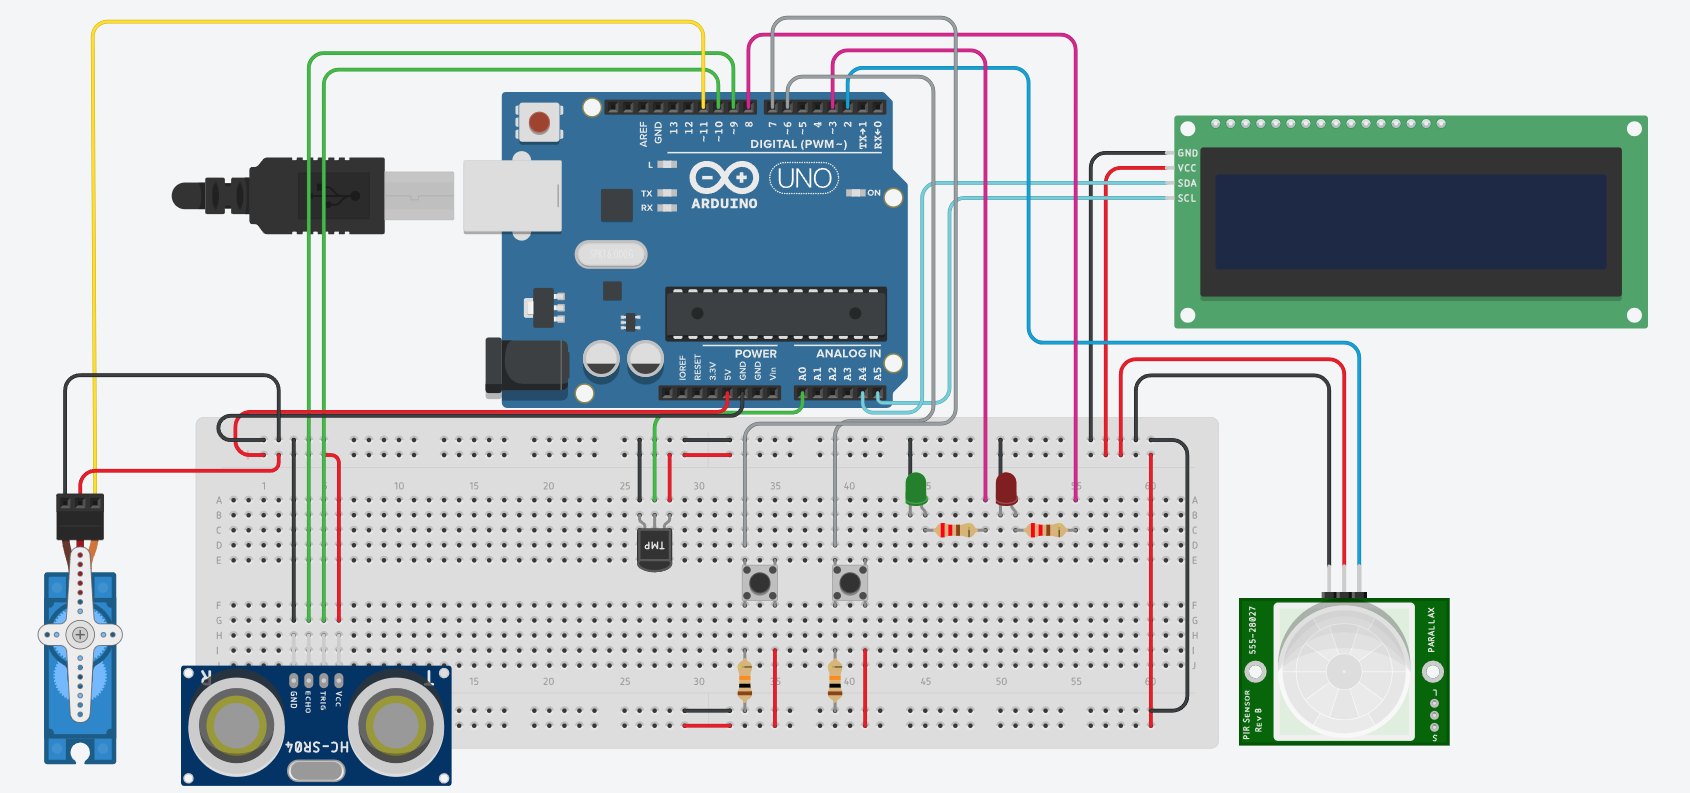
\includegraphics[width=\linewidth]{assignment-02/img/wiring.png}
    \caption{wiring del progetto}
    \label{fig:wiring}
\end{figure}

\end{document}
